Do sań o masie \emph{m} przyłożono siłę \emph{F} pod kątem \emph{$\alpha$}, jak na rysunku \emph{a}. Z jakim przyspieszeniem poruszają się sanie, jeżeli współczynnik tarcia wynosi \emph{$\mu$}? Z jakim przyspieszeniem będą się poruszać sanie, jeżeli siła \emph{F} zostanie przyłożona jak na rysunku \emph{b}, pod takim samym kątem \emph{$\alpha$}?
\begin{figure}[h]
	\centering
	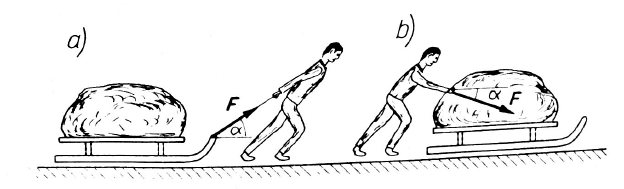
\includegraphics[width=0.3\linewidth]{../rysunki/dynamika/sanki-tarcie}
\end{figure}

%Kruczek 5_10R/49
%Poziom A